\documentclass[10pt, a4paper, egregdoesnotlikesansseriftitles]{scrartcl}


% initialize packages and macros
% general math/drawing stuff
\usepackage{geometry}
\usepackage{mathtools}
\usepackage{hyperref}
\usepackage[]{graphics}
%\usepackage{tikz}      -- see tikz section
%\usepackage{pgfplots}
\usepackage{amsmath, amssymb}

% Packages for algorithms/code -- copied, possibly unnecessary
\usepackage{listings}
\usepackage{verbatim}
\usepackage{algorithmicx}
\usepackage[noend]{algpseudocode}
\usepackage{algorithm}
\algdef{SE}[DOWHILE]{Do}{doWhile}{\algorithmicdo}[1]{\algorithmicwhile\ #1}%

% nicer author management
%\usepackage{authblk}

% colorsssss
\usepackage[dvipsnames]{xcolor}
% define your colors at the end

% drawing tools
\usepackage{tikz}
\usepackage{pgfplots}
\pgfplotsset{compat=1.16}
% add all required graph elements here
\usetikzlibrary{arrows.meta, automata, backgrounds, shapes, decorations}
\usetikzlibrary{positioning,fit,calc}  
\tikzset{
        block/.style={draw, thick, text width=3cm, minimum height=1.5cm, align=center},   
        line/.style={-latex}
    }

% useful common symbols idk copied em
\newcommand{\booleans}{\mathbb{B}}
\newcommand{\naturals}{\mathbb{N}}
\newcommand{\integers}{\mathbb{Z}}
\newcommand{\ordinals}{\mathbb{O}}
\newcommand{\numarals}{\mathbb{I}}
\newcommand{\reals}{\mathbb{R}}

\newcommand{\maps}{\rightarrow}
\newcommand{\pmaps}{\hookrightarrow}

\newcommand{\union}{{\cup} }
\newcommand{\Union}{{\bigcup} }
\newcommand{\powerset}[1]{2^{#1}}
\newcommand{\intersection}{{\cap} }
\newcommand{\intersect}{\intersection}
\newcommand{\Intersection}{{\bigcap} }
\newcommand{\compose}{{\circ} }


\newcommand{\ltrue}{\mathbf{tt}}
\newcommand{\lfalse}{\mathbf{ff}}
\newcommand{\limplies}{\Rightarrow}
\newcommand{\lxor}{\oplus}
\newcommand{\Land}{\bigwedge}
\newcommand{\Lor}{\bigvee}
\newcommand{\Lxor}{\bigoplus}
\newcommand{\lequiv}{\Leftrightarrow}
\newcommand{\landplus}{\mathrel{:\hspace{-3pt}\land\hspace{-3pt}=}}
\newcommand{\lorplus}{\mathrel{:\hspace{-3pt}\lor\hspace{-3pt}=}}
\newcommand{\bigO}{\mathcal{O}}


% author notes
\newcommand{\pushkar}[1]{{\color{Aquamarine} Pushkar: #1}}
\newcommand{\sankalp}[1]{{\color{RubineRed} Sankalp: #1}}


% colorssssss
\definecolor{test}{HTML}{FF0000}

% general macros go here
\newcommand{\petris}{\texttt{petris}}


% allow a figure to be broken across columns and pages
% its absence is a source of sheer annoyance - sg
\allowdisplaybreaks{}
\geometry{a4paper, textwidth=6.3in}

\title{$\petris$}
\subtitle{A Tetris Clone}

% Authors, ordered by roll num
\author{
    Pushkar Mohile \\
    $\texttt{180260027}$
    \and
    Sankalp Gambhir \\
    $\texttt{180260032}$
    }

\date{June 2020}

\begin{document}

\maketitle

\begin{abstract}
    \centering
    $\textbf{Abstract --}$
    $\petris$ is a bad attempt at a portmanteau of 
    EP and Tetris. We recreate the well known game of NES Tetris \cite{tetris}
    using Verilog, with simulations done using Verilator \cite{verilator} under
    a C++ wrapper with a VGA display simulator based on Simple DirectMedia Layer 2
    \cite{sdl2} running on an OpenGL based hardware-accelerated renderer. Our approach
    is innovative, using software layers to emulate nearly perfectly a set of
    physical buttons and a display output, alllowing for distinctive software-backed
    realtime play in the absence of an FPGA. The code is available publicly on our 
    GitHub repository \cite{petrisgit}.

\end{abstract}

% section names copied from the format from now, subject to change
  
\section{Project Details}
% description of block structure 
The design is structured into 3 main tiers (see Fig. \ref{fig:blockdiag} ),
the C++ wrapper (see \ref{subsection:cppwrap}), which handles clock
processing and display simulation, the Verilog wrapper (see \ref{subsection:wrapper})
which instantiates all lower tiered modules and acts as interfacing
media for them. The third and bottom-most tier is split into two 
main parts, handling game logic (see \ref{subsection:logicalmod}) and
display control (see \ref{subsection:display}) respectively.

% block diagram
\begin{figure}[ht]
    \centering
    
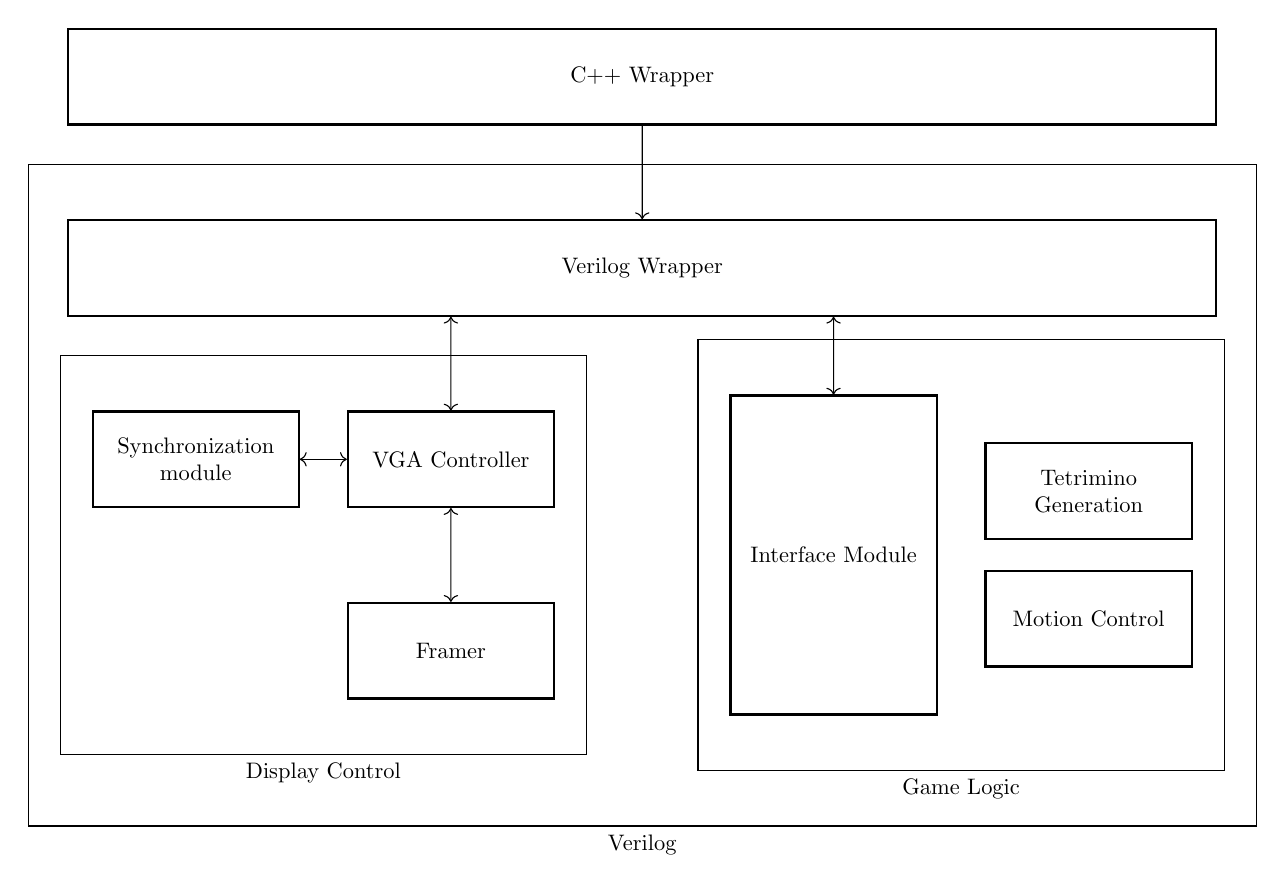
\begin{tikzpicture}[scale=0.81, every node/.style={transform shape}]
    % macro block diagram for simulation

    \node[block, minimum width=18cm ] (cpp) at ( 0,  0) {C++ Wrapper};
    
    % blocks part of the display super-module
    \node[block, minimum width=18cm ] (main) at ( 0, -3) {Verilog Wrapper};
    \node[block] (sync) at (-7, -6) {Synchronization module};
    \node[block] (vga) at (-3, -6) {VGA Controller};
    \node[block] (fr) at (-3, -9) {Framer};
    
    % blocks part of the logic super-module
    \node[block, minimum height=5cm] (int) at ( 3, -7.5) {Interface Module};
    \node[block] (tetgen) at ( 7, -6.5) {Tetrimino Generation};
    \node[block] (motcon) at ( 7, -8.5) {Motion Control};

    \node[draw,inner xsep=4mm,inner ysep=7mm,fit=(vga)(fr)(sync), label={-90:Display Control}] (d) {};
    \node[draw,inner xsep=4mm,inner ysep=7mm,fit=(int)(tetgen)(motcon), label={-90:Game Logic}] (l) {};
    
    \node[draw,inner xsep=4mm,inner ysep=7mm,fit=(main)(d)(l), label={-90:Verilog}] (v) {};

    % super-module connections
    \draw[->] (cpp)-- (main);
    \draw[<->] (vga)-- (vga|- main.south);
    \draw[<->] (int)-- (int|- main.south);

    % display connections
    \draw[<->] (vga.west)-- (sync.east|- vga.west);
    \draw[<->] (fr)-- (vga);

    % logic connections

\end{tikzpicture}

    %\captionsetup{justification=centering}
    \caption{Block diagram $\sankalp{Better\ caption?}$}
\label{fig:blockdiag}
\end{figure}

% verilog
\subsection{Verilog Structuring}

% wrapper
\subsubsection{Wrapper}
\label{subsection:wrapper}
%
\begin{lstlisting}[language=Verilog]
    input clock;
    input [3:0] actions; // input user action [ROTATE | DOWN | LEFT | RIGHT]
    output vsync;
    output hsync;
    output vga_r;
    output vga_g;
    output vga_b;
    output [7:0] score;
    output gameover;
\end{lstlisting}

Verilog modules are instantiated top-down for the purposes of the 
simulation. The logical structure of the design leaves us with 
several root modules, both harder to manage in practice, and 
unsupported as of yet for the purposes of simulation \cite{verilatortopmod}.
So we create a module that accepts inputs from the C++ wrapper (\ref{subsection:cppwrap}),
provides outputs to it, and acts as an interfacing media for the different
modules, with necessary root modules instantiated within this wrapper.\\

% logic supermodule
\subsection{Logical Modules}
\label{subsection:logicalmod}
\subsubsection{Structural Description of Gameboard}
\label{subsubsection:Structuraldescr}
\begin{lstlisting}[language=Verilog]
    input wire [4:0] operation,  
    input wire vsync, 
    input reg [10:0] framenumber, 
    output reg [2:0] currentstate[0:9][0:19], 
    output reg [7:0] score,
    output reg gameover,
    input clock
\end{lstlisting}
The logical module for the game consists of a single module that takes inputs from the top level wrapper and outputs the board state to the frame buffer. \newline
along with the gamescore and a gameover state. The \code{vsync} acts as the clock that drives the game.

Further, there are several internal components 
\begin{lstlisting}[language=Verilog]
    reg [2:0] tetrimino;
    reg frozen;
    reg [2:0] num_deleted;
    reg [4:0] centerofmass [0:1][0:3]
\end{lstlisting}
These parameters store the coordinates and type of the falling 
tetrimino and use it for tracking the position and state of the block.\\

\subsubsection{Interface}
\label{subsubsection:interface}
The instantiation of the module sets all the registers in the boardstate to 0. An initial tetrimino is generated.
\newline 
When the gameclock updates module performs certain tasks 
\begin{itemize}
    \item Check whether the current tetrimino is frozen or can move more
    \item If it is frozen, check whether the game is over checking whether any block of the top row is filled
    \item If the game isn't over, delete the rows that are filled, update the score ,move all rows above down, generate a new tetrimino
    \item If the tetrimino isn't frozen, move it down 
\end{itemize}
We faced issues issues with the syncing of the above actions and input due to the relatively low framerate of the clock. 
Therefore evaluating of the movement is instead done at \code{negedge vsync} to prevent inputs 
from being evaluated simultaneously with the above evaluations.
\subsubsection{Tetrimino Generation }
\label{subsubsection:tetgen}
The inital block is generated as a L-Block. 
Every subsequent block is generated based on the framenumber 
at which the generation happens, which ensures sufficient percieved 
randomness using a simple hashing
 \( \texttt{(Framenumber * PrimeNumber\ \%\ 7) + 1} \) 
With the center of mass at (0,5).
\subsubsection{Motion Control }
\label{subsubsection:motioncontrol}
4 operations are allowed
\begin{itemize}
    \item Move down
    \item Move left
    \item Move Right
    \item Rotate Clockwise
\end{itemize}
 A tempory set of coordinates is created based on the current coordinates of the tetrimino and the operation 
 \begin{itemize}
     \item If the operation is to move left, right or down, all the 4 blocks in the tetrimino are moved by 1 block in the appropriate direction
     \item If the operation is to rotate, the center of mass remains constant while the other 3 blocks rotate clockwise by 90 degrees around the center of mass
 \end{itemize}
 If the operation is found to be valid, the coordinates are updated to
 be equal to the temporary coordinates previously calculated and the boardstate is updated by deleting the blocks at the previous coordinates
 and creating a tetrimino at the new coordinates

\subsubsection{Validation }
\label{subsubsection:validation}
Two things are checked to see whether a move is valid 
\begin{itemize}
    \item Whether the new position goes beyond the boundary. 
    by checking  whether the coordinates are greater than 9 and 19 respectively
    \item Whether the new position overlaps with an occupied block. 
   
\end{itemize}

% display supermodule
\subsection{Display Modules}
\label{subsection:display}

\subsubsection{VGA Control Module}
\label{subsubsection:vgacontrol}
%
\begin{lstlisting}[language=Verilog]
    input clock;
    input reg [2:0] frame_buffer [0:9] [0:19], // frame [x][y][R | G | B]
    output reg [2:0] vga_pixel, // output bus for 3-bit RGB color
    output hsync_out;
    output vsync_out;
\end{lstlisting}

The VGA control module serves as a generator for the serial VGA output 
(ports 3-5) and instantiates the framer (\ref{subsubsection:framer}) and
the synchronisation module (\ref{subsubsection:vgasync}).

Every \(\texttt{vga\_clock}\) (see \ref{subsubsection:vgasync}), based on the
current \(\texttt{count\_x}\) and \(\texttt{count\_y}\), the relevant pixel from \\
\(\texttt{frame\_buffer}\) is outputted to the VGA bus.\\
 

\subsubsection{Framer Module}
\label{subsubsection:framer}
%
\begin{lstlisting}[language=Verilog]
    input vsync;
    inout reg [2:0] frame_buffer [0:9] [0:19];
    output reg [2:0] frame_out [0:9] [0:19];
\end{lstlisting}

The Framer Module maintains a frame buffer with controlled public access,
gated using a semaphore \cite{semaphore}. This allows other modules and tasks 
to write directly to the frame buffer instead of maintaining copies of the data 
potentially causing overwriting and synchronisation issues.

The module writes this frame buffer onto an output buffer at \(\texttt{vsync}\), 
in turn sent onto VGA rails serially (\ref{subsubsection:vgacontrol})
over the course of the next frame cycle. After flushing this data, the buffer is cleared,
i.e. written over with black, preparing it for the next output cycle.\\

\subsubsection{Synchronisation Module}
\label{subsubsection:vgasync}
%
\begin{lstlisting}[language=Verilog]
    input clock;
    output vga_clock;
    output hsync;              
    output vsync;               
    output in_display;          
    output reg [9:0] count_x;
    output reg [9:0] count_y;
\end{lstlisting}

The Synchronisation Module receives a \(\texttt{clock}\) signal from
the VGA controller (\ref{subsubsection:vgacontrol}) and calculates several
signals critical to the VGA control flow:

\begin{itemize}
    \item \(\texttt{vga\_clock}\) --- a signal generated by dividing the 
            input \(\texttt{clock}\) signal by a known \(\texttt{multiplier}\)
            variable. The multiplier variable can be easily adjusted at runtime
            to allow for adjusting frame times in the event of a performance
            bottleneck or sudden throttle to prevent a drop in frametimes. This
            is akin to a primitive version of modern Adaptive Syncing \cite{varrefresh},
            now popularized as some technologies built into modern GPUs,
            such as AMD Freesync \cite{freesync} and Nvidia G-Sync \cite{gsync}. 
            Modern implementations instead use a specialised controller on the display
            side as well, communicating actively with its counterpart in the GPU,
            as opposed to our host-only solution.
    \item \(\texttt{vsync / hsync}\) --- sync signals standardized as part of the VGA
            standard \cite{vgastandard}. Intended to be passed via a DAC to the monitor.
            In our implementation, \(\texttt{hsync}\) sees little use other than this,
            while \(\texttt{vsync}\), marking, the end of a frame, is at several points 
            (\ref{subsubsection:interface}, \ref{subsubsection:motioncontrol}, \ref{subsubsection:framer}, 
            \ref{subsection:cppwrap}) used to flush a frame buffer or to advance a logical step.
\end{itemize}


% c++
\subsection{C++ Wrapper}
\label{subsection:cppwrap}

In the absence of an FPGA to run described modules, 
we had to look to other options. With a strong desire to 
maintain real-time playability, we tried several options ---
standard simulations had to be rejected due to not being 
anywhere close to real-time, with the inability to accept inputs.
Having considered the idea of running a simulated clock, we then
moved to forcefully driving a clock for the simulation.
\\
\\
 We attempted to use \(\texttt{verilog-vga-simulator}\) \cite{vga-simulator},
a C-based program interfacing with the simulation via 
Verilog Procedural Interface (VPI) \cite{vpi}, drawing the resultant
VGA output via Simple DirectMedia Layer \cite{sdl2} referred to as 
SDL herein. We were driven away by a cocktail of issues --- primarily
the performance, combined with the relative inflexibility of VPI 
and the now obsolete SDL API. However, the cocktail
was more than resolvable. 
\\
\\
Our saving grace came in the form of Verilator \cite{verilator}, a compiler for
Verilog which translates modules top-down into C++ code with
I/O interfaces handled via classes \cite{verilator-implement}. This allowed
us to bypass having to deal with VPI's idiosyncrasies and limited nature, paired
with the finicky fixes required to obtain a realtime driven clock.
\\
\\
Armed with a way to handle inputs and outputs to our modules in realtime, we 
needed a VGA simulator to handle the outputs. This was executed using
SDL2 and a low-level frame-buffer, rendering to screen via 
a cross-platform hardware accelerated rendering interface (with OpenGL \cite{opengl}
primarily used for testing).

\begin{figure}[h]
    \centering
    \includegraphics[scale=0.6]{fig/ouput_screenshot.png}
    \caption{SDL based output}
\label{fig:output}
\end{figure}

However, a software based simulation is unable to drive a clock fast enough
to run a VGA simulation in any of the common modes \cite{vga_modes}. As such,
a myriad of performance-centric changes had to be made. Alongside several
minor optimizations was a major change to the system --- a drastic reduction in
resolution or frame rate. Realistically, keeping the same resolution, the frame 
rate would have been cut to approximately \(\texttt{1/20 fps}\), far from playable.
The resolution would have to be cut similarly to maintain a playable frame rate.
Since most of our clock cycles are used up driving the VGA controller, keeping true
to the design, we chose to downscale it. Outputting a much smaller resolution from
the simulated Verilog modules and writing an integer scaling \cite{intscale} system
within the relatively fast C++ wrapper. 
\\ \\
We would like to add that much higher raw resolution and frame rates are possible 
and have been seen after removing the limitation to output serial VGA. Providing
the frame buffer as output to the display simulator in parallel reduces the time
complexity of drawing a frame from \(\bigO (n^2)\) to \(\bigO (1)\) in screen 
dimensions. However, having achieved desired levels of responsiveness and 
playability without resorting to bending the limits of the project, we chose not 
to do this.

\section{Main Components}

The physical components to develop this project would be 
\begin{itemize}
    \item An FPGA
    \item A VGA Display
    \item A DAC to feed the output of the FPGA to the VGA
    \item Buttons to control the inputs 
    \item A laptop with the Intel Quartus software and the required connecters. 
\end{itemize}}

\section{Credits and Mistakes}
In the process of writing this report, we discovered that \(\texttt{vga-sim}\)
by ZipCPU \cite{vgasimzip} implements a similar Verilator based approach. We had
already developed our own system with great difficulty and dozens of cycles of 
trial and error for achieving the same goal by the time we discovered it. Their
software, offered as both an open-source and commercial product, is vastly superior 
in terms of raw display capability, and is very well written. Having a similar 
original model, we decided not to switch despite possible performance gains, as well
as for other reasons, notably it not implementing an input system similar to ours.
We have not had a chance to fully explore its display capabilities due to time
constraints, but we would recommend it wholeheartedly. Despite the troubles,
it was a great experience for us, so we are proud of our flawed system.
We felt they still deserved credit here for developing the technology, and we hope
less people in the future in similar proedicaments will miss this software, 
for the hard work of the people at ZipCPU, as well as the sanity of they
who try to implement it themselves \(\textsf{;)}\)  

\section{Results}
The game works as intended with the operations being correctly evaluated
 and the gameboard updating correctly to reflect all the changes. The score updates correctly on deletion of full rows, with greater weights 
being given to deleting more rows simultaneously. The game correctly ends on any coloumn being filled. \\
A quick gameplay run showing this can be seen in the folllowing video: \\
 https://drive.google.com/drive/folders/1vZAzBuaDIm5yseN7SvnVuGAI3CmcGi4w?usp=sharing

\\
There are several optimizaions and additional features that can be implemented. Implementations to the User Interface could include
\begin{itemize}
    \item A game reset button that allows you to play multiple games on one execution
    \item A high score display that keeps track of your best performances
\end{itemize}} 
Potential optimizations to the game would include
\begin{itemize}
    \item Improving the framerate of the VGA simulator
    \item Introducing more parallel updating for the game logic, which it is currently not due to synchronization and framerate issues. This currently doesn't matter 
     due to the low framerate being the rate determining step but this should definitely be done if using a real FPGA 
\end{itemize}}



\end{document}